\chapter{Identifying and Optimizing Base Classifiers for Various Feature Types}\label{ch:varFeat}

Data sets may have many different kinds of features: besides floating point numbers, integers and Booleans,
they often also contain single characters or whole character strings.
Often times one data set even contains features of different data types.

\begin{figure}[ht]
    \centering
    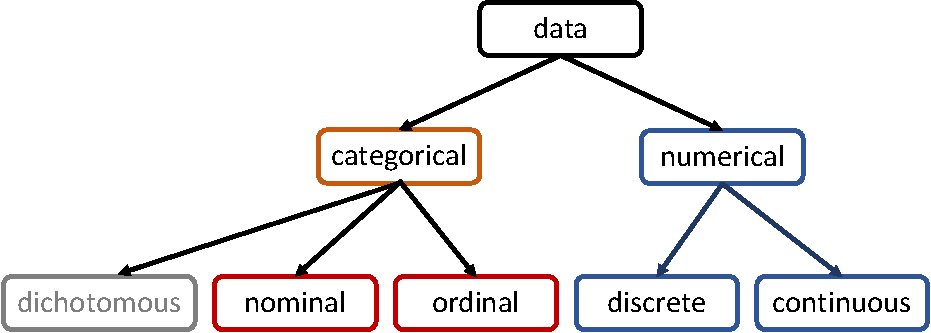
\includegraphics[width=\columnwidth]{figures/data_classes.pdf}
    \caption{Hierarchy of the different data types~\citep{brownlee,dahouda}.}\label{fig:dataClasses}
\end{figure}

% Types of Data
The most common approach is to group data into categorical and numerical types, as seen in \autoref{fig:dataClasses}.
While numerical data is represented in the form of numbers, categorical data is usually represented by character strings.
Continuous variables are real-valued floating point numbers that are defined over uncountable sets of values like \(\mathbb{R}\).
Discrete variables, in contrast, are defined over countable, finite sets of values and are required to have a one-to-one correspondence to \(\mathbb{N}\).
Ordinal variables, like \(\text{size} \in \{\text{S, M, L}\}\), have embedded orderings,
whereas nominal variables, like \(\text{color} \in \{\text{red, green, blue}\}\), do not have such underlying hierarchies.
Moreover dichotomous variables, also known als binary variables, have exactly two distinct values~\citep{brownlee, dahouda}.

% the SCM handling numerical variables
Numerical variables are easy to process for most machine learning algorithms.
In particular, the SCM with data-dependent rays is defined on numerical data and can handle both, continuous and discrete variables, effortlessly.
Due to the natural limitation of features values, caused by the finite amount of samples, every feature dimension is essentially discrete.
This enables the uniform processing of continuos, as well as discrete, variables within the SCM.\

% ML algorithms fail on categorical features
Even though categorical features are very common in real-world problems, 
many machine learning algorithms are not capable of processing raw text as an input for their features~\citep{dahouda,potdar}.
Often times those categorical features first need to be encoded into numerical ones, in order to be processed.
~\cite{dahouda} introduce some very advanced encoding mechanisms, however, such encoding usually still
involves a loss in performance of the classification algorithm,
the need of an increased amount of features, as well as a loss of the data's expressiveness,
and should therefore be avoided.

% the SCM handling nominal and mixed variables
As nominal variables have no embedded ordering and therefore rules like `color >= blue' make no sense,
nominal features cannot simply be transformed into numerical
features and need to be handled in a separate routine.
A dichotomous variable can, and will in this thesis, also be handled as a nominal variable with the small value range of size two.
This has the advantage that is allows the variable to not only be a Boolean, but any kind of binary
value set, like for example \{fast, slow\}.
Therefore the SCM's routine, of looking for the best possible base classifier on each feature, is split into two:
One routine to examine a numerical feature (see \autoref{sec:numerical}) and one to examine a nominal feature (see \autoref{sec:nominal}).

% the SCM handling ordinal variables
The SCM could furthermore handle ordinal variables either like nominal variables, but paired together with an order relation~\citep{dahouda},
or they can be parsed, together with an explicit notation of their underlying order relations, into a discrete variable.
However I decided not to support ordinal variables, as the implementation is quite
unspectacular and I do not want to make the code unnecessarily complex.
Additionally, it is sometimes even beneficial to manually convert ordinal variables into discrete numeric ones,
for example by substituting \texttt{\{child,teenager,senior\}} for \texttt{\{5,15,65\}},
as this gives the user the chance to include semantics that would have been lost otherwise,
like `teenager' being closer to `child', than to `senior'.

The final SCM can now not only deal with floating point numbers and integers by applying a routine for numerical features,
but also handle character strings --- and consequently even Booleans and single characters
as those are parsed into character strings implicitly by the Julia mechanics.
On these raw text features the algorithm then applies a routine for nominal features.
It is moreover by-default possible for this modified SCM to analyze data sets with mixed feature types,
provided that each feature is of one distinct type.
This works, as the SCM with such single threshold base classifiers assesses each feature dimension independently and is therefore
able to handle inconsistent feature types effortlessly~\citep{schmid}.
This enables mixed type rules like `\texttt{IF color = black AND radius >= 2.5 THEN wheel}' that barely any other machine learning algorithm is able
to produce as easily, as the SCM does.

Julia generally recognizes the type of each feature, i.e.\ the data type of the feature's column within the data frame, automatically.
It only needs a little help for parsing strings from CSV files, as displayed in \autoref{julia:loadCsv}.
My SCM then works with the data types `\verb|const NumericalFeature = Union{Vector{Float64}, Vector{Int64}}|'\\
and `\texttt{const NominalFeature = Union\{Vector\{Bool\}, Vector\{String\}\}}'.\\
When examining a feature for high scoring base classifiers, the algorithm now employs multiple dispatch to use one function
on all nominal features and another function on all numerical features.
A data set might for example resemble the one in \autoref{tab:mixed_data}.
The features types were added by Julia automatically, initially it was a plain CSV file.

\begin{table}[ht]
    \centering
    \caption{Data set with mixed feature types.}\label{tab:mixed_data}
    \begin{tabular}{l|lllll}
        Row & x1 & x2 & x3 & x4 & label \\
         & Float64 & Int64 & Bool & String & Int64 \\
        \midrule
        1 & 0.1323 & 15 & false & red & 0 \\
        2 & 0.7046 & 127 & true & blue & 0 \\
        3 & 0.2139 & 9 & false & purple & 1 \\
        4 & 0.5103 & 300 & true & white & 1 \\
        5 & 0.1685 & 111111 & false & green & 0 \\
        6 & 0.699 & 210 & false & orange & 1 \\
        7 & 0.374 & 16 & false & red & 0 \\
        8 & 0.08105 & -50 & false & blue & 0 \\
        9 & 0.7964 & 17 & false & purple & 1 \\
        10 & 0.0954 & -3 & true & purple & 1
    \end{tabular}
\end{table}

%%%%%%%%%%%%%%%%%%%%%%%%%%%%%%%%%%%%%%%%%%%%%%%%%%%%%%%%%%%%%%%%%%%%%%%%%%%%%%%%%%%%%%%%%%%%
\section{Locating Optimal Base Classifiers on Numerical Features}\label{sec:numerical}

To find and evaluate data-dependent rays on a numerical feature the procedure in \autoref{code:numerical} is executed.
Here the SCM first looks for a border to delimit the feature from above, then from below and finally it returns the optimum of both.
This leads to a total number of \(2 \cdot |\text{samples}| \cdot |\text{numerical features}|\) possible rays that need to be evaluated.
However in fact not every sample will have a different value for this feature and therefore
the algorithm's `featureVector' can be reduced by removing all its duplicates.
This reduces the total number of possible rays to only \(2 \cdot |\text{unique sample-feature values}| \cdot |\text{numerical features}|\).

\begin{algorithm}[ht]
    \KwIn{featureVector, labelVector, \(p\)}
    \For{featureValue \(\in\) featureVector}{
        Calculate the usefulness score of the ray `feature \(\leq\) featureValue' using \autoref{julia:calcScore}.
    }
    upperBorder = ray of this loop with the maximum usefulness score \\
    \For{featureValue \(\in\) featureVector}{
        Calculate the usefulness score of the ray `feature \(\geq\) featureValue' using \autoref{julia:calcScore}.
    }
    lowerBorder = ray of this loop with the maximum usefulness score \\
    Return the border with the higher usefulness score.
    \caption{Basic algorithm to determine the optimal ray on a certain numerical feature.}\label{code:numerical}
\end{algorithm}

% Optimization: Clever Score Calculation
This algorithm can be heavily optimized: the result will be the same, yet the execution time can be
decreased from \(\mathcal{O}(|\text{samples}|^2)\) to only \(\mathcal{O}(|\text{samples}|)\),
enabling the SCM to process even huge data sets, such as the gene expressions in \autoref{sec:geneticData}.
Instead of considering the feature value of every sample for the score calculation of a possible threshold,
the optimized algorithm iterates through all samples only once and calculates the current positions's scores based
on the last positions's score, without needing to check every sample in a nested loop.

The algorithm, that is depicted in \autoref{julia:inspectNumerical}, then works as follows:
First all values that the samples have at this feature component are collected, duplicates are removed
and the final vector is sorted from low values to high values.
Each of these possible thresholds then gets assigned two numbers: the number of positive samples that
have this value as its feature component and the number of negative samples that do so.
Afterwards the lower and upper border are again calculated and the optimal border is returned.
Yet, this time an optimized algorithm, illustrated in \autoref{julia:findBorder}, is used.
This new algorithm based on the fact, that Q and R always only change by the number of positive and negative samples that had the
last threshold as their feature value.
As the possible thresholds are ordered from low to high, the optimal lower
border is located first, in order to use the fact that both, Q and R, of the ray `\(x \geq \text{minValue}\)' are always 0,
as every sample is placed within this ray.
The analog fact also applies to the ray `\(x \leq \text{maxValue}\)', which is why the vector
of all possible thresholds is reversed before looking for the optimal upper border later on.

Starting from \(Q=R=0\) for the first threshold, the values of the next threshold can be calculated by
\[Q_{new} = Q_{old} + |\text{`negative samples at the previous threshold'}|\]
\[R_{new} = R_{old} + |\text{`positive samples at the previous threshold'}|\]
For example in the case of \autoref{fig:lowerBorder}, the algorithm starts on the very left
with \(Q=R=0\) and continues to advance to the right with \(Q=0\)  \(R=1\), \(Q=1\) \(R=2\) and so on.
Regarding the upper border on the reversed threshold vector, this also works in the same way.
On the same data, the algorithm this time starts on the very right
with \(Q=R=0\) and then proceeds with \(Q=1\) \(R=0\), \(Q=3\) \(R=0\) and so on (see \autoref{fig:upperBorder}).
A single threshold classifier's score is then, as always, deducted by \(Q - p \cdot S\).

\begin{figure}[ht]
    \centering
    \begin{subfigure}{\textwidth}
        \centering
        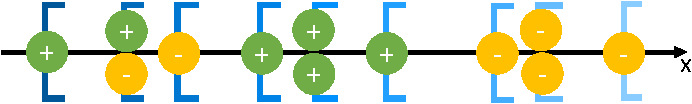
\includegraphics[width=0.85\columnwidth]{figures/lower_border.pdf}
        \caption{Advancing from left to right to evaluate possible lower borders.}\label{fig:lowerBorder}
    \end{subfigure}
    \hfill
    \begin{subfigure}{\textwidth}
        \centering
        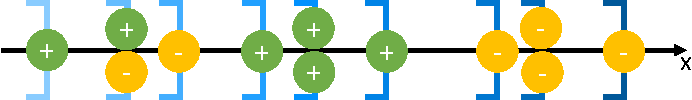
\includegraphics[width=0.85\columnwidth]{figures/upper_border.pdf}
        \caption{Advancing from right to left to evaluate possible upper borders.}\label{fig:upperBorder}
    \end{subfigure}
    \caption{Iteration through a feature vector to locate optimal borders.}\label{fig:borders}
\end{figure}

%%%%%%%%%%%%%%%%%%%%%%%%%%%%%%%%%%%%%%%%%%%%%%%%%%%%%%%%%%%%%%%%%%%%%%%%%%%%%%%%%%%%%%%%%%%%
\subsection{Dealing with the Re-correction of Rays}

% the situation
The SCM is choosing one ray after another and adds them to the conjunction.
However it often also chooses rays that have the same feature-operator combination as a previously selected rule.
This leads to rules like `\texttt{IF x1 < 5 AND x1 < 3}', where the first ray is basically `re-corrected'.
The re-correcting ray will always be tighter than the first one, since the conjunction
algorithm deletes all positive samples outside the chosen rays in every iteration,
making it impossible that rays with thresholds outside those previous conjunctions are selected afterwards.
Moreover re-correcting will never happen on nominal features, as all other threshold regarding this feature
are immediately outside of the conjunction, once a base classifier regarding this feature is chosen.
To illustrate this, the rule `\texttt{IF x2 = blue AND x2 = red}' can be taken into account, that will always evaluate to `false'.

\begin{figure}
    \centering
    \begin{subfigure}{\textwidth}
        \centering
        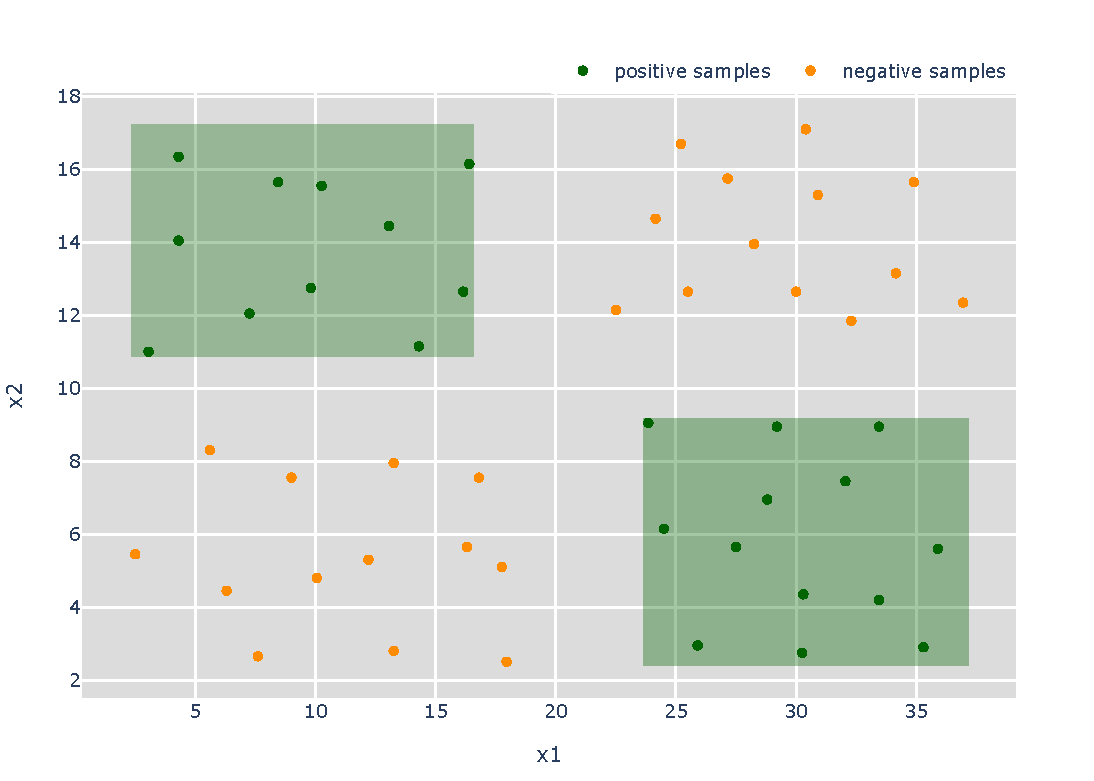
\includegraphics[width=0.85\columnwidth]{figures/two_reg_recorrecting.pdf}
        \caption{Re-correcting allowed.}\label{fig:withRecorr}
    \end{subfigure}
    \hfill
    \begin{subfigure}{\textwidth}
        \centering
        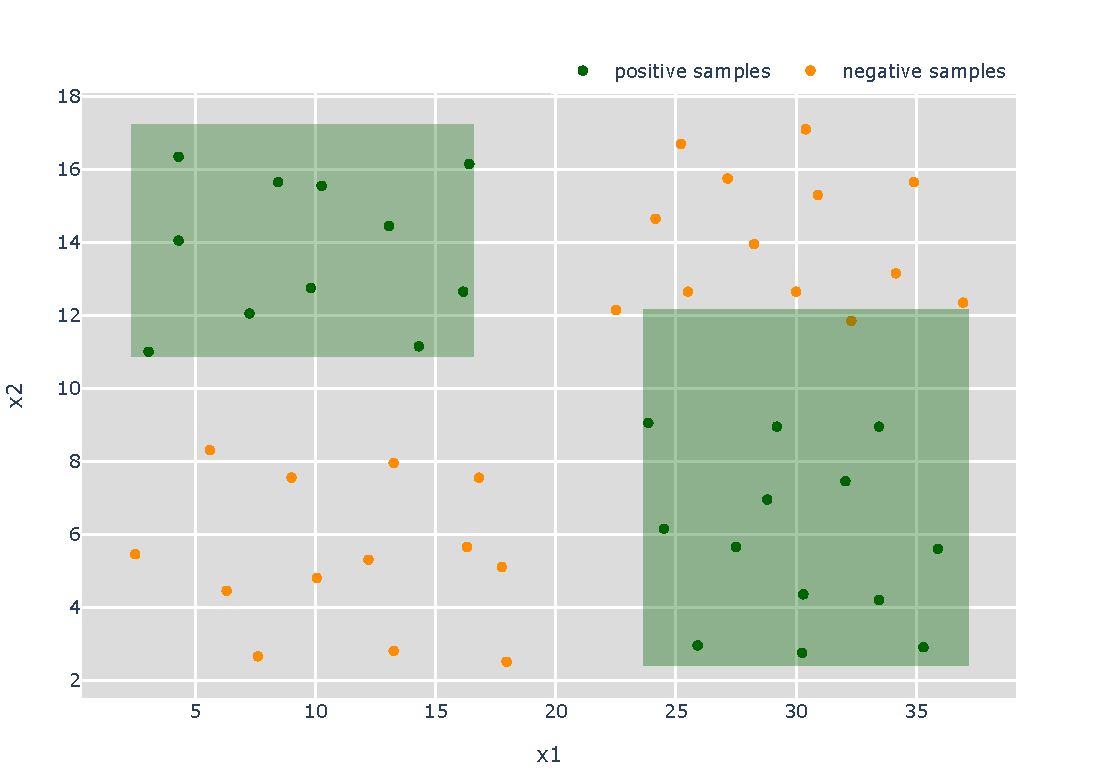
\includegraphics[width=0.85\columnwidth]{figures/two_reg_no_recorrecting.pdf}
        \caption{Re-correcting prevented.}\label{fig:noRecorr}
    \end{subfigure}
    \caption{Classification rule for an artificial data set with two disjunct decision regions.
        In both cases \(p\) is set to 1.2 and \(minConjSize\) to 1.}\label{fig:recorr}
\end{figure}

% how to prevent re-correcting
The process of re-correcting may be prevented by placing the code block of \autoref{julia:preventRecorr} in front of
the usefulness score computation of every ray, to ensure that rays, that would otherwise re-correct
previously chosen rays, will not be selected.
Yet this re-correcting behavior is in general a good thing, as it usually improves the algorithms results,
like in the example of \autoref{fig:recorr}, by reducing the decision region within the rays
to a better size, now that the SCM with data-dependent rays knows the new, more limited, region.
Additionally, as \autoref{tab:geneCompact} illustrates, the chance of actually deciding to re-correct
when working in a big feature space is actually really small.
Yet in order to prohibit the overriding of rays, many parameters need to be parsed down to low-level functions.
So in the common case of having many features and therefore usually not even considering to re-correct, having
the `feature' to prohibit re-correcting, slows down the whole SCM.\

% conclusion
Therefore I allow the SCM to re-correct previously made ray choices and
include the line `\texttt{filter!(r -> r.featureId!=ray.featureId || r.operator!=ray\\.operator, selectedRays)}'
to the end of the \texttt{build\_conjunction} algorithm, to delete the overridden ray.

%%%%%%%%%%%%%%%%%%%%%%%%%%%%%%%%%%%%%%%%%%%%%%%%%%%%%%%%%%%%%%%%%%%%%%%%%%%%%%%%%%%%%%%%%%%%
\subsection{Placing Thresholds Right in between Data Points}

When using a character to store a numerical ray's direction, the direction can be more than just the binary `\(\geq\)' and `<', as suggested by~\cite{kestler11}.
In this chapter so far the operators `\(\leq\)' and `\(\geq\)' were used for rays
and therefore the thresholds were placed directly on positive samples, like in \autoref{fig:thresholdMin}.
However when using `<' and `>', the thresholds will always be placed on negative samples, as in \autoref{fig:thresholdMax}.
A third option, that will be used from now on, is to place a threshold directly in the center
between the two involved data points, like in \autoref{fig:thresholdMiddle}.

\begin{figure}[h]
    \centering
    \begin{subfigure}{\textwidth}
        \centering
        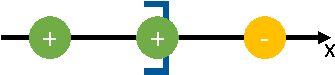
\includegraphics[width=0.5\columnwidth]{figures/threshold_min.pdf}
        \caption{x \(\leq\) 2.}\label{fig:thresholdMin}
    \end{subfigure}
    \hfill
    \begin{subfigure}{\textwidth}
        \centering
        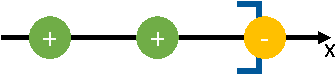
\includegraphics[width=0.5\columnwidth]{figures/threshold_max.pdf}
        \caption{x < 3.}\label{fig:thresholdMax}
    \end{subfigure}
    \hfill
    \begin{subfigure}{\textwidth}
        \centering
        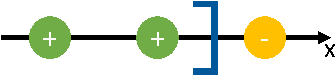
\includegraphics[width=0.5\columnwidth]{figures/threshold_middle.pdf}
        \caption{x < 2.5.}\label{fig:thresholdMiddle}
    \end{subfigure}
    \caption{Possible rays to correctly classify three data points.}\label{fig:variousThresholds}
\end{figure}

This variation can be implemented by extending the method to find a ray on a single numerical feature, depicted in \autoref{julia:inspectNumerical},
with the output of `winnerRay', by an additional functionality that shifts the rays threshold.
So far this threshold is placed directly on the positive sample, with the next sample on the ray's
negative side being a negative one, as a threshold is always placed on the smallest or largest positive sample within an area~\citep{schmid}.
This threshold shifting is generally defined as
\[threshold_{new} = \frac{threshold_{old} + \text{`value of sample next to the ray's negative side'}}{2}\]
and the result will be rounded to two decimals, in order to receive compact thresholds.
However, when trying to process a ray in the form of `\(x \geq \text{minValue}\)' or `\(x \leq \text{maxValue}\)',
there is no more sample on the negative side of the ray and the algorithm, that is furthermore
portrayed in \autoref{julia:thresholdInbetween}, therefore does not modify those rays.

By the definition of~\cite{kestler11} a ray is only considered as data-dependent, if its threshold is directly placed on a sample value.
Therefore the SCM is now per definition dealing with data-independent rays, even though those thresholds do clearly depend on the sample's components.
Additionally the placement of thresholds in between samples comes with the downside that, in case
of integer features, the thresholds might not be integers anymore, but floating-point numbers.
Therefore the rays will not necessarily be located in the feature domain.

However, by placing the threshold in the center of two samples, the ray's margins towards the samples are maximized.
Thus, this version of the SCM is expected to have a lower generalization error~\citep{shawe}.
In data sets like \autoref{fig:tightLooseThr}, the placement of thresholds between samples visibly
does increase the ability of the model to generalize, yet in data sets with many samples, like the gene expressions in \autoref{sec:geneticData},
these improvements are often only marginal, as the large amount of feature values leads to
small gaps between two samples and therefore only small differences between classification
rules with thresholds on and between samples can be identified.

\begin{figure}
    \centering
    \begin{subfigure}{\textwidth}
        \centering
        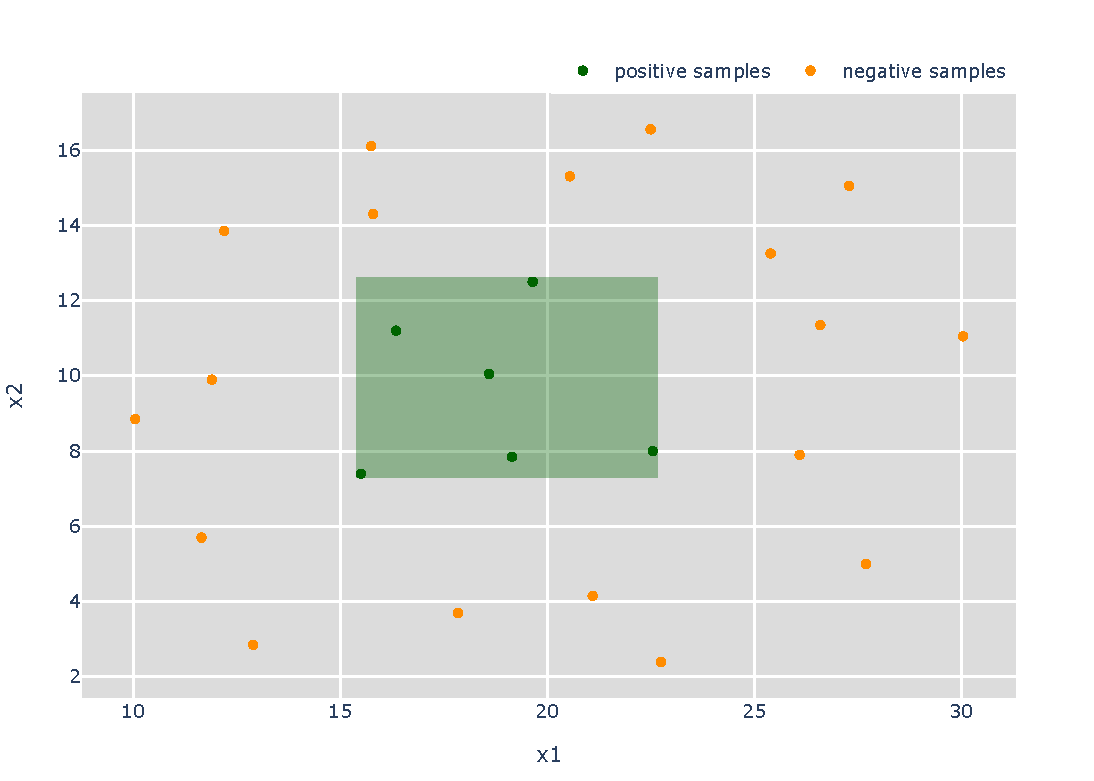
\includegraphics[width=0.85\columnwidth]{figures/one_reg_tight.pdf}
        \caption{Setting tight bounds by placing the thresholds directly on the positive samples.}\label{fig:tight}
    \end{subfigure}
    \hfill
    \begin{subfigure}{\textwidth}
        \centering
        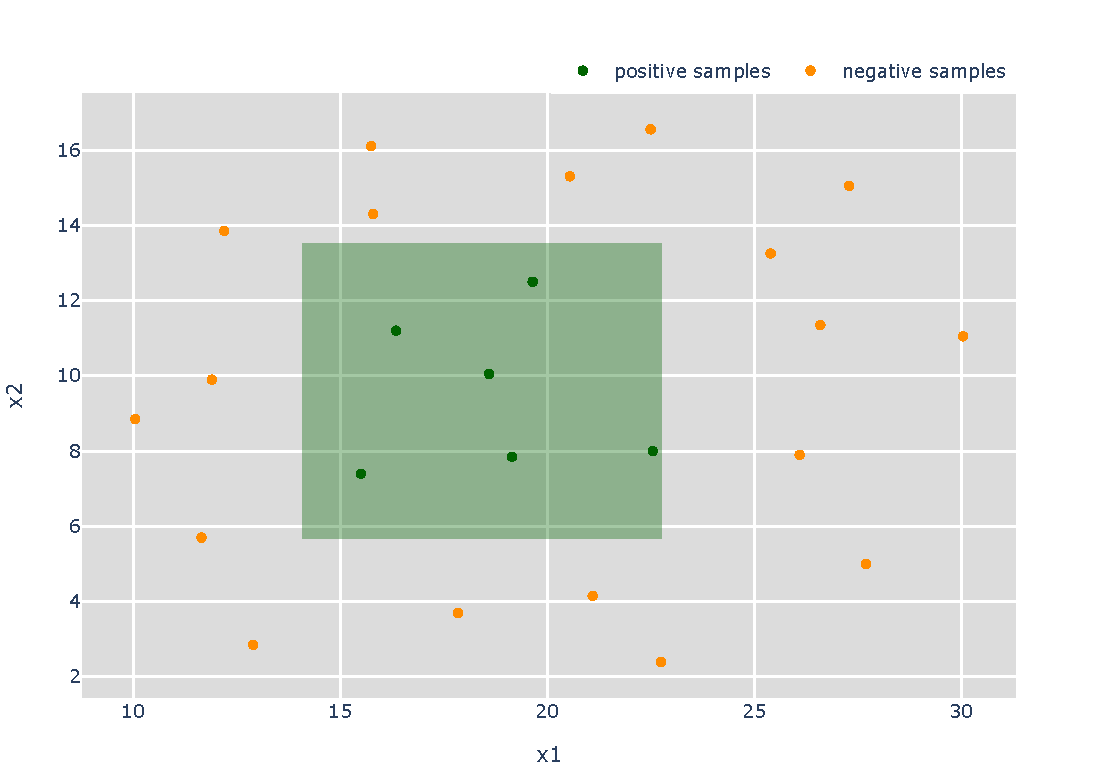
\includegraphics[width=0.85\columnwidth]{figures/one_reg_loose.pdf}
        \caption{Setting loose bounds by placing the thresholds in the centers between positive and negative samples.}\label{fig:loose}
    \end{subfigure}
    \caption{Classification rule for an artificial data set with one central decision regions.
        In both cases \(p\) is set to 3 and \(minConjSize\) to 1.}\label{fig:tightLooseThr}
\end{figure}

After all, as the new thresholds do not classify any of the training samples
differently than the previous version of the algorithm does,
the selection of the next rays is not effected by this design choice.
Therefore the other properties of the classifier, like its number of rays, will in general
be the same as before.

%%%%%%%%%%%%%%%%%%%%%%%%%%%%%%%%%%%%%%%%%%%%%%%%%%%%%%%%%%%%%%%%%%%%%%%%%%%%%%%%%%%%%%%%%%%%
\section{Locating Optimal Base Classifiers on Nominal Features}\label{sec:nominal}

The SCM is moreover extended by a routine that computes the optimal base classifiers on nominal features.
Those can be determined, by executing the algorithm portrayed in \autoref{code:nominal}.
This algorithm simply checks and compares the usefulness scores of classifiers that each limit one feature to one of its sample values.
Analog to the algorithm on nominal features, the duplicates values within the feature vector can be removed to speed up the algorithm.

\begin{algorithm}[ht]
    \KwIn{featureVector, labelVector, \(p\)}
    \For{featureValue \(\in\) featureVector}{
        Calculate the usefulness score of the classifier `feature = featureValue' using \autoref{julia:calcScore}.
    }
    Return the base classifier of this loop with the maximum usefulness score.
    \caption{Basic algorithm to determine the optimal base classifier on a certain nominal feature.}\label{code:nominal}
\end{algorithm}

Two extensions, that are deliberately not implemented, are the `\(\neq\)' and the `\(\in\)' operator.
A `\(\neq\)' operator for nominal features, as in `\texttt{IF x \(\neq\) green THEN class 1}', is not realized in order not to make the algorithm unnecessarily complex.
Features with small value ranges, and especially binary features, do not need a \(\neq\) operator in the first place.
Also, a disjunction of base classifiers on the same feature like \texttt{`x = red OR x = blue OR x = purple'}
is not joined into a set like `\verb|IF x in {red, blue} THEN class 1|', since pure disjunctions like this very rarely, if at all, happen within the \(SCM_{DNF}\).\
Particularly on data sets with many features and an \(sC > 1\), the chance of at least two such
single classifiers of the same feature to appear within the DNF is basically non existent.

% Optimization
Furthermore the complexity of \autoref{code:nominal} is reduced by one dimension, as the last dimension's
Q, R and consequently also its usefulness score, can be deducted from the previous ones:

\[Q_z = |\text{`negative samples'}| - \sum_{i=1}^z Q_i\]
\[R_z = |\text{`negative samples'}| - \sum_{i=1}^z R_i\]

With \(z\) being the last dimension, for example \(z=2\) in the case of a binary feature.
The full implementation, which requires the algorithm from \autoref{julia:calcScore}
to return Q and R additionally to the usefulness score, can be found in \autoref{julia:inspectNominal}.
Testing on the data sets of \autoref{sec:uci} revealed that this new algorithm actually really
improved the SCM's runtime by a bit, as displayed in \autoref{tab:nominalFast}.

\begin{table}[ht]
    \centering
    \caption{Execution times of a \(10 \times 10\) cross-validation using different algorithms for nominal features.}\label{tab:nominalFast}
    \begin{tabular}{lllll}
        \toprule
        & \multicolumn{2}{c}{unoptimized} & \multicolumn{2}{c}{optimized} \\
        data set & execution time & RAM & execution time & RAM \\
        \midrule
        chess & 1.445~s & 4.47~GiB & 1.299~s & 3.82~GiB \\
        german & 0.678~s & 1.43~GiB & 0.672~s & 1.29~GiB \\
        \bottomrule
    \end{tabular}
\end{table}